\documentclass[ notitlepage, numerical, 11pt]{revtex4-1} % style for Physical Review B and AJP are similar
\usepackage{float}
\usepackage{amsmath}

\usepackage{graphicx} 


\usepackage{sverb}

\begin{document}

\title{Physics of Data Storage}
\author{Tenzin Rigden}
\affiliation{Carleton College, Department of Physics, Northfield, MN 55057}
\date{\today}
\begin{abstract}
Being able to store your personal data is an incredible scientific acheivement already. However,  more and more of our lives are getting digitized( whether its our music, games, and even textbooks). Beacuse of thi it is important to D only learn how our current techniques to store data work, but it is also important to learn what new techniques are being uncovered to help us store more data in the future.
Word count: 4936
\end{abstract}

\maketitle
\section{Introduction}
Since we live in the information age, computers are a ubiquitous part of our lives. Just as important as the computer itself is what's stored in it. Your pictures, music, videos, papers, and more are all stored on a computer. As more and more of our lives begin to live digitally, it has become increasingly important to find new ways to either expand our current data storage technologies or find new ones. On a fundamental level, a computer stores everything in a series of 1s or 0s called bits. In this binary system, 1 represents a "true" state while a 0 represents a "false" state. This binary system can be represented in nearly anyway to store data from "yes hole" or "no hole" in punch cards to "yes current" or "no current" in transistors. 

In this paper, I will talk about the different techniques that are currently being used for long-term storage, non-volatile memory. I will also, when possible, talk about the advancements already made in that field to increase storage size and current research being done to further increase it. Lastly, I will talk about modern techniques currently being developed that could greatly increase storage size.



\section{Optical Storage}
\subsection{Optical Disks}
Optical disks have been commonplace for a long time in the United States. While optical disks aren't typically the preference for storing data directly from the computer, they are frequently used transwr inceca For optical disks, data is recorded and read using a laser beam. To record data, a laser beam is shone on the reflective surface creating a pit with a depth of the wavelength of the laser divided by 2. Thus lands are the areas that were not shone on by the laser. To read, a very low power laser is shone on the disk and the reflected signal is converted to an electrical signal using a scanning photo detector. A "1" is interperted as when there is a change in the surface, i.e. changing from pit to land or land to pit, and a "0" is interperted as when there is no change in the surface. The way this is manifested is that when at a changing point for the surface, the laser will be shining at both the land and the pit. This means that the light reflected off of the pit will have a phase change of $\lambda/2$ behind the light reflected off of the land causing destructive interference and no reflected light, "1". When there is no change in the surface, the light simply reflects back normally and is interpreted as a "0" \cite{memory}.

\begin{figure}[H]
\centerline{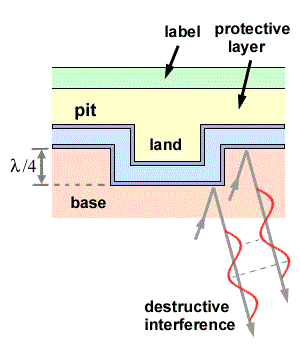
\includegraphics[scale=.9]{cdRom.png}}
\caption{ This is a cross-sectional view of a CD-ROM where there a pit signifies a $\lambda/4$ depth meaning when a laser shines over a change from land to pit or vice versa, destructive interference will take place signifying a bit value of 1.}
\label{cdRom}
\end{figure} 
Optical Disks come in a few different styles: Compact Disk ROM (CD-ROM), CD-Recordable (CD-R), CD-Rewriteable (CD-RW), and Digital Versatile Disk (DVD). These disc technologies are written sequentially in a continous spiral track eminating from the middle out. This causes it to be slower than other technologies that use cocentric tracks. A CD-ROM is a disc that's only meant to be readable and typically used for things such as installation of programs. Since it is only written once in the factory, a glass master disk is created using a high intensity laser. Liquid polycarbonate is inserted into the master disk to recreate the disk which is then covered with a reflective layer then a protective one. 
A CD-R is slightly different because it needs to be able to written to once outside of the factory. This is one by having a painted layer between the reflective layer and transparent layer. The painted layer is initially transparent and becomes dark to simulate a pit when impacted by a high-intensity laser. Lastly, in a CD-RW, the reflective layer has two states, a slightly reflective amorphous state and a highly reflective crystalline state. A high intensity laser shone on this layer will cause it to turn into its amorphous state and simulates a pit, while a medium intensity laser will cause it to change back into its crystalline state and simulates a land. And again, a low intensity laser is used to read the pits and lands without affecting the state.

\begin{figure}[H]
\centerline{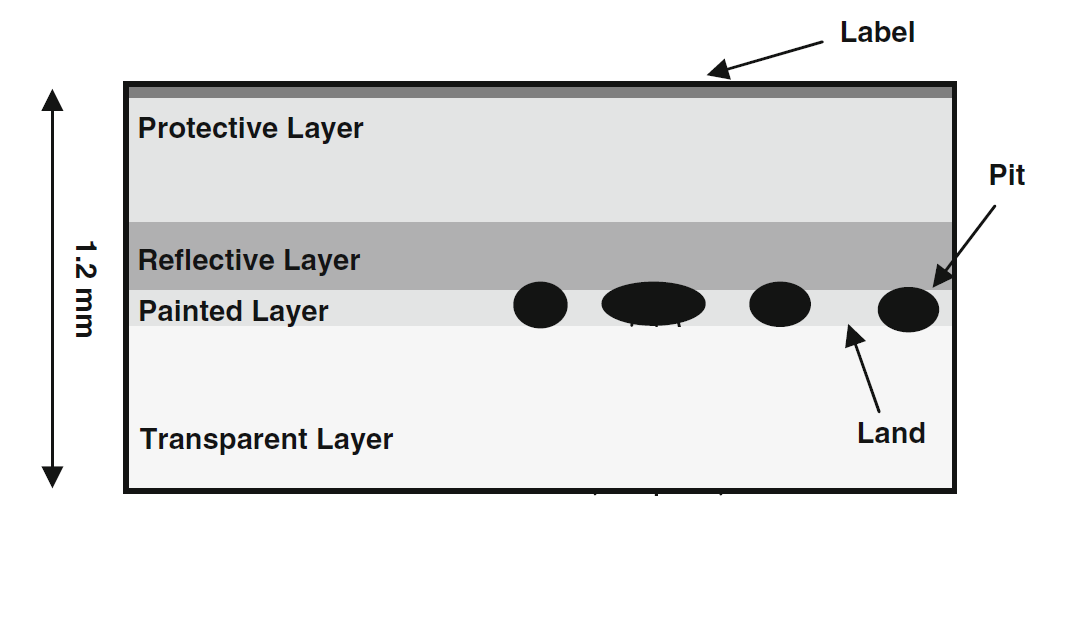
\includegraphics[scale=.45]{cdR.png}}
\caption{In this cross sectional view of a CD-R, the painted layer, if shone on by a high intensity laser will develop dark spots simulating pits.}
\label{cdR}
\end{figure} 

While CDs were useful and easy to carry around, their size was limited to only 700MB. Demand for higher storage capacities in the 1990s led to the invention of the DVD which offered data storage of at least 4.7GB. The first main difference between CDs and DVDs is that DVDs use a shorter wavelength light, 650nm, than CDs use, 780nm. What this allows is that pits and lands in the DVD can be much smaller and can be placed closer together than a CD could, increasing storage density to about 2.2Gb/in$^2$ from .9Gb/in$^2$. Another innovation that allowed storage of up to 8.5GB was the ability to have two different recording layer: a semi reflective layer in the middle and a fully reflective layer at the other end. The different layers can be read by changing the focus of the laser. Additionally, instead of having a protective layer on one side of the disk, you can put another disc on it to effectively double the capacity again. However, this requires the manual flipping of the disc when accessing the other half of the data. By having double sided and a double layer, DVDs can achieve a storage of 17GB \cite{memory}.

\begin{figure}[H]
\centerline{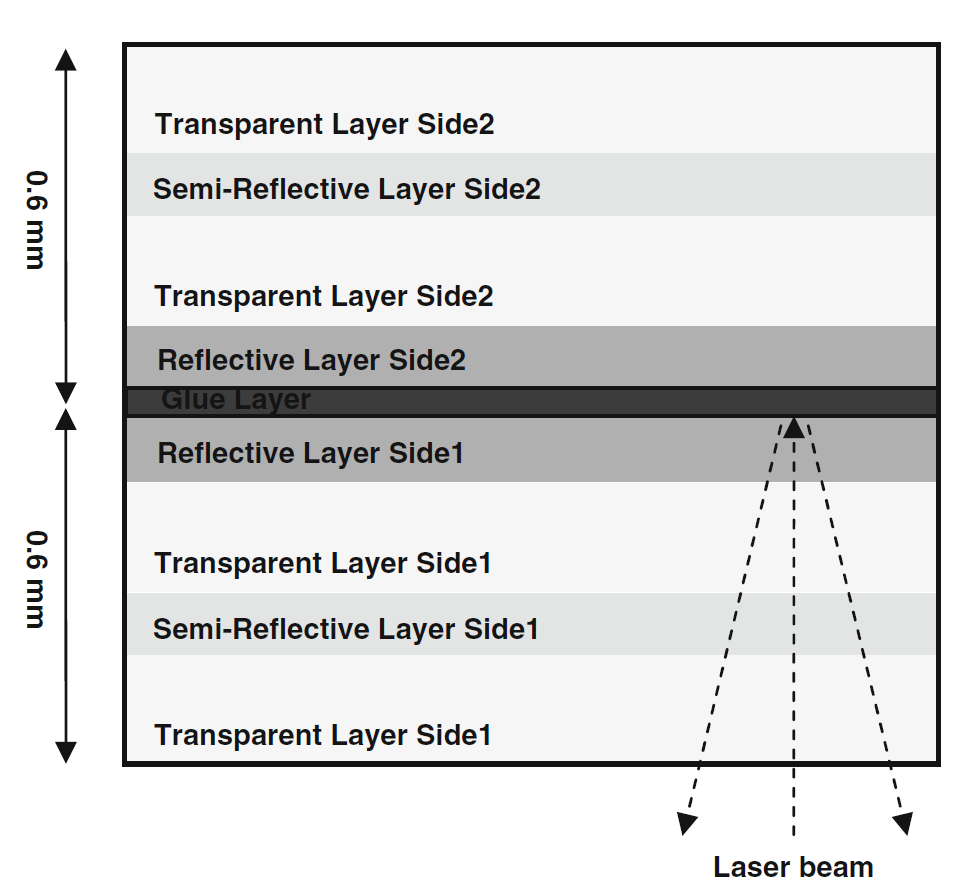
\includegraphics[scale=.45]{DVD.png}}
\caption{This is a cross section of a double sided and dual layer DVD. The pit and land information is stored at the two reflective and semi-reflective layers. The layer in which the laser is reading from is selected by focusing the laser to for that layer depth. To access the other side of the DVD, it must be physically removed and placed upside down.}
\label{DVD}
\end{figure} 

A more recent innovation in storage of optical disks was the invention of the Blu-ray disc. Just like how using a smaller wavelength light in DVD compared to the ones in CD allowed the reduction in size of the pits and track size, Blu-ray discs also use a much smaller wavelength light to increase capacity. Blu-ray uses 405nm light which allows both the pit sizes and the track size, space between tracks, to be reduced to .15$\mu$m and .32$\mu$m respectively compared to the track size of .74$\mu$m for DVDs. This allows a storage density of 2.2Gb/in$^2$ to be achieved. 



\subsection{Holographic Data Storage}
However, these all still pale in comparison to the potential storage capabilities of holographic data storage (HDS) of over 1Tb/in$^2$. In the most basic sense, a holography is the method of capturing and recreating optical information through interference patterns. To record a hologram, a coherent light source is split into a reference and object beam using a beam splitter. The object beam is reflected off the object being recorded on to the photographic plate. The reference beam, also being shone on to the photographic plate, experience interference with the object beam and that interference pattern is recorded on the plate as a hologram. Destructive interference appears as dark spots and constructive interference appears as bright spots. This can all be seen in Figure \ref{create}. 

\begin{figure}[H]
\centerline{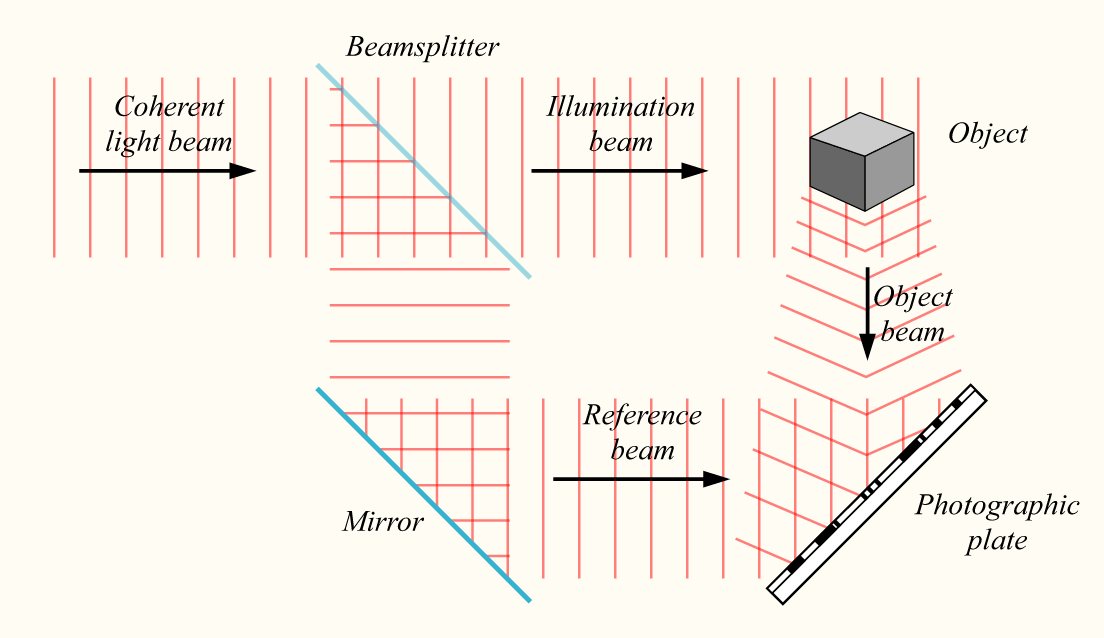
\includegraphics[scale=.45]{create.png}}
\caption{This is an example of a transmission hologram where a coherent souce of light is split into a reference beam and an object beam. The two beams eventually create an interference pattern at the photographic plate creating a hologram. }
\label{create}
\end{figure} 

To recreate the image from the hologram, the reference beam is shone back at the hologram at the same angle and by looking at where the object should be through the hologram, a virtual image can be seen of the object as seen in Figure \ref{reconstruct}.

\begin{figure}[H]
\centerline{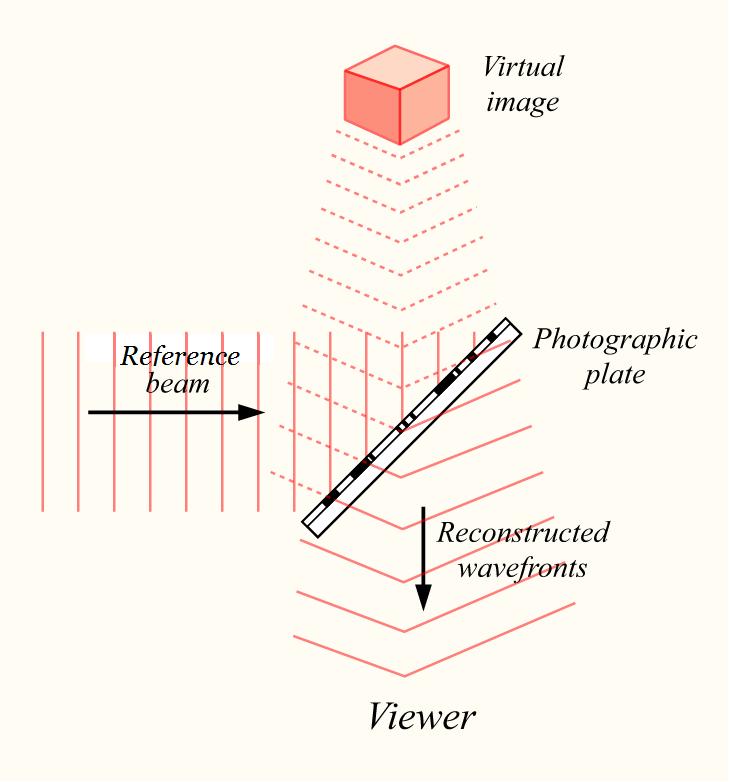
\includegraphics[scale=.45]{reconstruct.png}}
\caption{To recreate the virtual image, the reference beam is shined on the hologram at the same angle, and by looking through the hologram to where the object should be, a virtual image can be seen.}
\label{reconstruct}
\end{figure} 


Holograms can be created in both thick and thin regimes. The thin regime is unsuitable for high density storage because thin holograms like those written on photographic film confine their diffractive interaction to a single plane and can't be used for multiplexing \cite{HDS}. The criterea used quantify the thickness or thinness of a hologram is known as the $Q$ parameter. The $Q$ parameter is given by 
\begin{equation}
Q = \frac{2\pi\lambda L}{n_0\Lambda^2},
\label{qParameter}
\end{equation}
where $\lambda$ is the wavelength of the light, $L$ is the thcikness of the recording layer, $n_0$ is the index of refraction of the medium, and $\Lambda$ is the grating period. A hologram is considered in the thin regine if its $Q$ parameter is $Q<1$ and is considered in the thick regime if its $Q$ parameter is $Q>1$. The thickness of the medium can range from 500$\mu$m to a few millimeters \cite{HDS}.

To store digital data in holograms, a spatial light modulator (SLM) is needed. The SLM converts the 1s and 0s of the digital data into light and dark pixel respectively in a pattern. The number of bits that can be stored per SLM image can be over one million, but this varys with the SLM. So to record digital data, instead of reflecting the object beam off of the object, it is shone through the SLM then onto the storage medium as seen in figure \ref{dataHologramCreate}. 

\begin{figure}[H]
\centerline{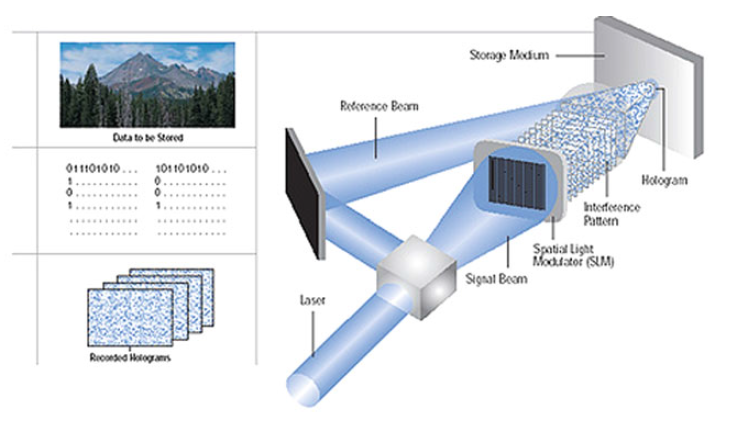
\includegraphics[scale=.45]{dataHologramCreate.png}}
\caption{This implementation of holographic storage uses the same technique as a transmission hologram except instead of reflecting the object beam off of the object, it is shone through the SLM which contains the bit information. Since the SLM page contains many bits at once, it can write more than one bit at once unlike magnetic drives.}
\label{dataHologramCreate}
\end{figure} 
Reading the hologram is the same as it would be for a thin hologram. The reference beam is shone at the hologram, but now there is a detector array to convert the SLM image of dark and bright spots into 1s and 0s for the computer. Since a page of bits can be read/written all at once at the speed of light instead of bit by bit, HDS has the ability to have much greater read write speeds over other competing technologies such as magnetic data storage.
\begin{figure}[H]
\centerline{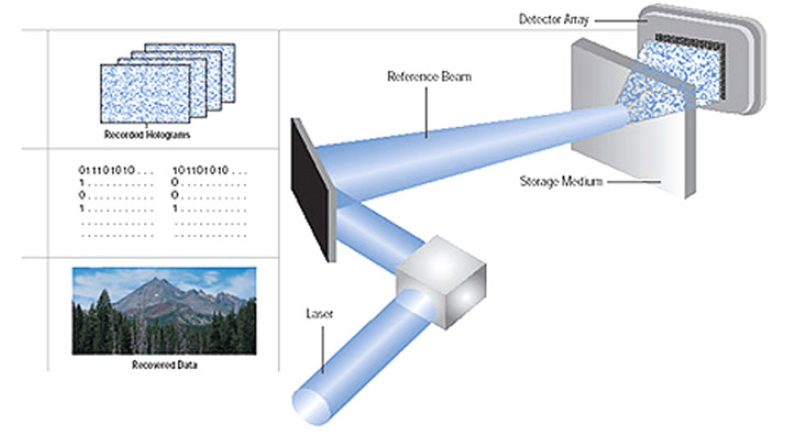
\includegraphics[scale=.45]{dataHologramReconstruct.png}}
\caption{Reading information is the same as recreating a hologram except now the virtual image is shone onto a detector array which converts the dark and bright spots into "1s" and "0s".}
\label{dataHologramReconstruct}
\end{figure} 
The reason why HDS can be so dense is because of the various multiplexing methods available. One type is angular multiplexing. Since the angle of the reference beam must match exactly the angle it had when recording the hologram, that means that a small change in the angle when recreating the image will cause the image not to appear. We can use this sensitivity by having one page of data from the SLM stored at one angle and by changing the angle of of entry. Another method to add multiplexing is to vary the wavelength of the the source and reference beams. This method is limited due to the small tuning range of lasers. Yet another method is to vary the point of entry of the beams into the medium. While there are more methods of multiplexing, the true benefit of multiplexing occurs when combining multiple multiplexing techniques at once. For example, hybrid wavelength and angular multiplexing systems have been tested before \cite{memory}. 


\section{Magnetic Storage}
\subsection{Background}
Another popular technology used to store data is magnetic storage. Though it is available in both tape and disk, I will only talk about disk here. Magnetic storage is a property can be attributed to the ferromagnetic property of certain metals such as iron and cobalt. Ferromagnetic materials are divided into small magnetic domains each with their own magnetic field in a direction. An unmagnetized ferromagnet will have these domains in random directions such that the net effect is 0 as seen in Figure \ref{domain}a. However, if an external magnetic field is applied, these domains will align with the external field and will stay aligned even after the external field is removed as in Figure \ref{domain}b.

\begin{figure}[H]
\centerline{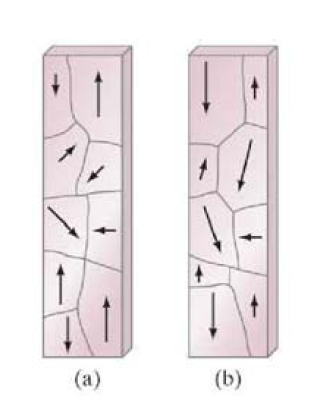
\includegraphics[scale=.45]{magneticDomain.png}}
\caption{Figure a represents an unmagnetized piece of iron where the domains are randomly oriented. Figure b represents where the domains are preferentialy aligned down.}
\label{domain}
\end{figure} 
This is due to the hysteresis loop experienced by the ferromagnetic material. If we start with an unmagnetized ferromagnetic material with no external magnetic field, point a in Figure \ref{hysteresis}, and increase the external magnetic field, $B_0$, we get to point b where there is a both a nonzero external amgnetic field and total field from the external and material. If the external magnetic field is then decreased to zero, instead of returning to point a, it instead reaches point c. Here, even though there is no external magnetic field, there is still an internal field from the ferromagnetic material. This phenomenom is what allows magnetic storage to store bits. A bit value of "1" is read when there is a reversal of current measured meaning that the magnetic field between two domains has swapped. A bit value of "0" is read if there is no change in the magnetic field and thus no change in the direction of the current measured.

\begin{figure}[H]
\centerline{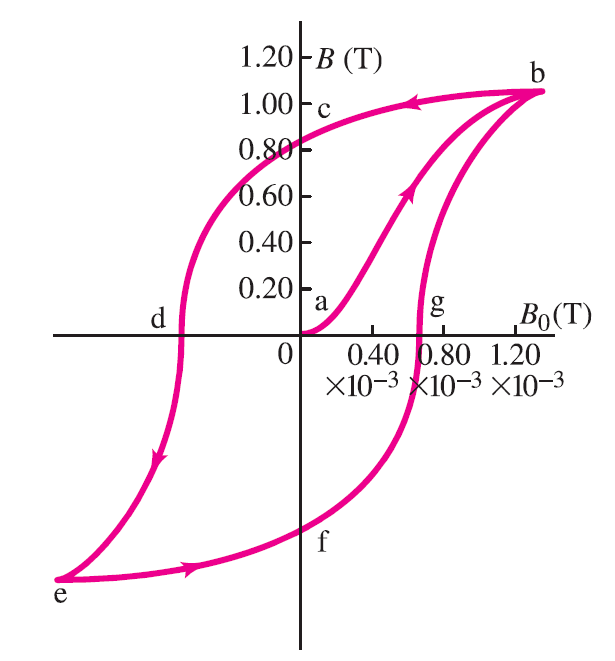
\includegraphics[scale=.45]{hysteresis.png}}
\caption{This displays a hysteresis loop of a ferromagnet. Following from point a, as an external field is applied, the total field reaches point b. As the external field is reduced to 0, since the ferromagnet partially keeps it alignment, a nonzero magnetic field exists even without an external field.}
\label{hysteresis}
\end{figure}

Reading and writing to the material is done by inducing a magnetic field using a head and coil of wire. The mechanics behind this are governed by Maxwell's equations. The two relevant equations are
\begin{equation}
\nabla x E = -\frac{\partial B}{\partial t},
\label{faraday}
\end{equation}
which is known as Faraday's law of induction and 
\begin{equation}
\nabla x B = \mu_0 J +\mu_0\epsilon_0\frac{\partial E}{\partial t},
\label{ampere}
\end{equation}
which is known as Ampere's law \cite{purcell}. Faraday's law tells us that a changing electric field will yield and changing magnetic field, and Ampere's law tells us the opposite. 

\subsection{Magnetic Disk Storage}
A magnetic disk drive is the most commonly used data storage technology used in consumer products today. First introduced in 1956 by IBM, modern drives consist of mainly of a read/write head and a hard platter with a ferromagnetic layer. Originally, the head was used for both reading and writing but compromises had to be made. The read head wants a thicker gap to be better able to penetrate the medium while the write head wants a smaller gap to get better accuracy. As domains got smaller, it became more and more difficult for the read/write heads to be able to properly read the intended domain from the increasing noise of the other domains. Nowadays, reading is done instead by a giant magnetoresistive (GMR) head. Magnetoresistance (MR) is the property that when a coiled wire will not only generate an electric field/current, it will also experience a change in resistance. This change in resistance can be used as a more accurate way to read the bits by applying a constant potential across a MR sensor and recording how the potential changes due to the change in the resistance of the wire because of Ohm's law. GMR is similar to MR but actually is a quantum effect. It is appropriately named because of its ability to change the resistance is giant in comparison to MR \cite{highDensity}. 


A GMR head consists of an antiferromagnetic exchange film (FeMn) and is used to pin the Co layer magnetization in a certain direction. Then there is the ferromagnetic Co layer called the pinned layer. After this is a copper spacer layer. Last is the second ferromagnetic layer called the free layer. So to start the two ferromagnetic plates have non-parallel magnetic fields causing the resistance experienced by a connected wire to be very high. When an external magnetic field is applied by say the bit being stored, the two ferromagnetic layers will align to the same direction of the external and thus the resistance will greatly drop. The mechanism behind this goes goes into the spin state of the moving electrons. These electrons can only have one of two possible states, up or down. If the spin states align with the direction of the magnetic field, they move forward in the wire simulating a lower resistance. However, if the spin state is against the field, then the electrons will travel in the opposite direction of the current causing more collisions and thereby increasing the resistance of the wire \cite{highDensity}.

The innovation of GMR read head and a dedicated write head allowed the domain bits to shrink even more. However, a new issue began to arise. The ability to retain stored data in the material is dependent on the product of $K_u$ and $V$ where $K_u$ is the magnetic anisotropy constant of the material. This product gives the energy barrier that must be overcome that allows the material to keep its magnetic field even without the external field. However, as the domains decrease in size to increase density, the volume decreases and so does the energy barrier. If the volumte of the domain decreases to the point where this energy barrier is around 60 times the manitude as thermal energy, $K_bT$, the domain may randomly switch its field direction and "flip bits." This created a limit to the storage density that longitudinal recording could attain \cite{perpendicular}.

To surpass this limit, the orientation of the recorded magnetic field changed from longitudinal recording to perpendicular recording. In addition to the change in orientation, the writing head was changed to a single-pole head and a highly permeable soft underlayer(SUL) was added below the recording material. The permeability of the SUL allowed it to act as a magnetic mirror to the actual head. This greatly increased the induced magnetic field used to write data. The stronger magnetic field means that materials with higher anisotropy values could be used that were not feasible for the weaker magnetic field in longitudinal recording. Because the anisotropy constant can be increased, the volume of the domain can be decreased further without worrying about thermal fluctuations. With all the above innovations, current HDDs can achieve a storage density of around 500Tb/in$^2$, but that continually seems to be increasing as scientists approach the limit.

\begin{figure}[H]
\centerline{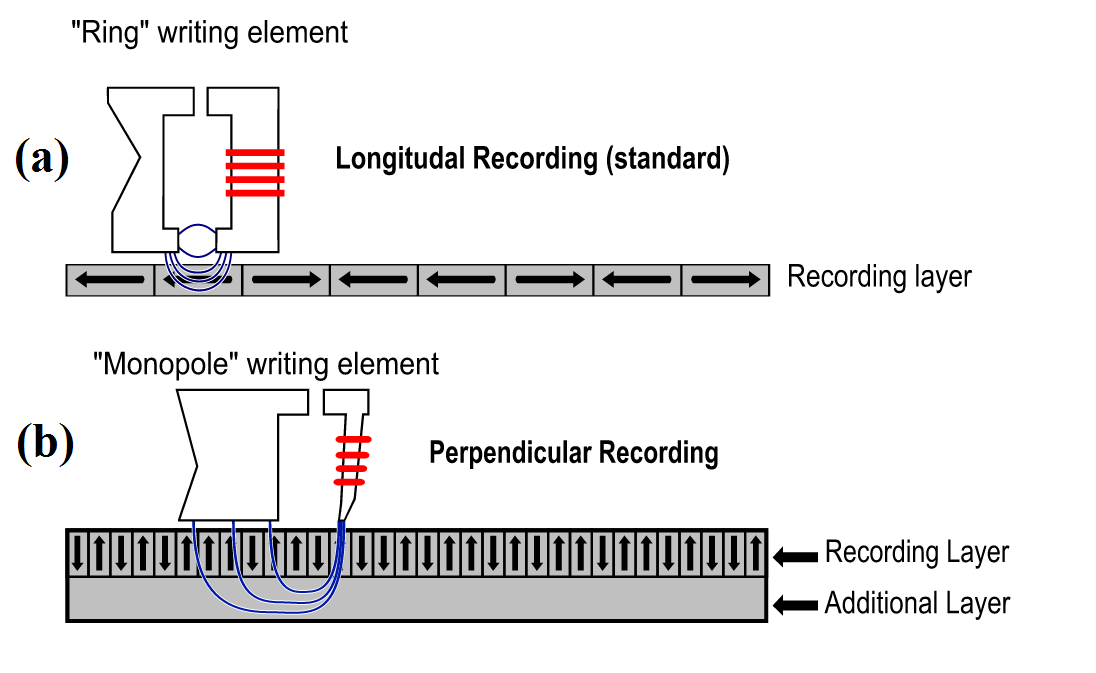
\includegraphics[scale=.45]{perpendicularComparison.png}}
\caption{Perpendicular recording due to the presence of the additional layer, soft underlayer, a much larger magnetic field can be applied to the recording layer. This allows us to use material with higher anisotropy meaning the domain size can be reduced and density increased.}
\label{perpendicularComparison}
\end{figure}


However, this too will have a limit at a smaller domain size where thermal fluctuations will be an issue again. One method still currently in development is called heat-assisted magnetic recording (HAMR). This method is based on the fact that all ferromagnetic materials have a curie temperature where the internal magnetic field it had is reduced to zero, and in the presence of an external magnetic field will align itself with that field. In HAMR, when a bit needs to get written to, a laser is used to heat up the desired domain to the curie temperature allowing our magnetic field to allign the domain, and then allowing the material to cool back down. This means that the recording material can be changed to one with a much higher anisotropy value allowing the domain sizes to decrease even more, further increasing the storage density \cite{hamr}.

Another potential way to push off of the thermal fluctuation barriar is through use of bit patterned media (BPM). The key to being able to surpass the thermal fluction limit is to have BPM make V from our equation large by cutting a magnetic layer to the size of one bit \cite{btm}.  Thus we can continue to decrease the size of our bit and increase our density. While this idea has been around since the 1990s, it has yet to take off because it was too expensive. However noe, the progress in lithography will soon make it vaible for BPM economically viable to come to market. BPM can also play a role in solving a potential issue in HAMR as well. HAMR has one issue where when heating up a bit locally, it could potentially heat up an adjacent bit cause it to reach curie temperature , and lose its data. BPM could potentially solve this issue by using a matrix with a low heat conductivity material. If successful, BPM has the potential to deliver storage densities of over 10 Tb/in$^2$!


\section{Flash Memory}

One of the most, if not the most, important device in modern computing as a whole is the transistor. A transistor is able take in a circuit input and act as a switch turning another circuits on or off without any moving parts. This ability to switch off and on a circuit will prove crucial in saving bits of memory.

\subsection{Semiconductors}
To explain how transistors work, first we need to explain what a semiconductor is since a transistor is a semiconductor device. A semiconductor is any material that are more conductive than insulators but less conductive than conductors.  A bandgap diagram is useful in describing semiconductors. Band structure represents the specific energy levels that electrons can occupy due to quantum mechanics. However, only the valence band is relevant when discussing conductivity. The valence band is the highest energy levels that electrons can occupy at absolute zero temperature. As seen in Figure \ref{bandGap}, the conductor is any material whose valence band is not completely full because it overlaps with the next higher energy band. This means that the valence electrons are free to move around and can carry a current. An insulator is any material whose conduction band is separated by a large band gap from its valence band. This means that the valence electrons can not easily move to its conduction band and thus are not free too move. Lastly, a semiconductor is any material whose conduction band is only separated by a small gap meaning that valence electrons can easily be excited into the conduction band and carry a current.


\begin{figure}[H]
\centerline{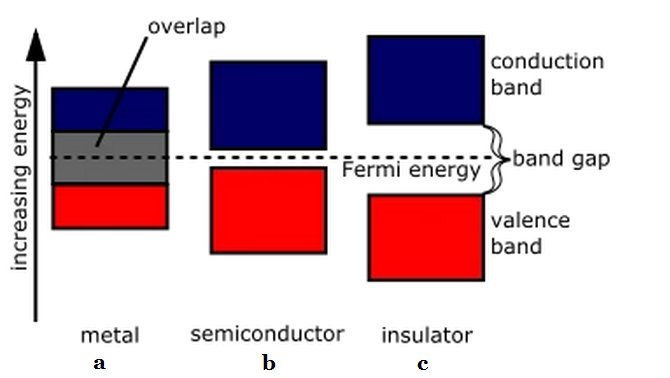
\includegraphics[scale=.45]{bandGap.png}}
\caption{Metals, a, are materials which have their valence electrons are free to move in the overlapping conduction band. Insulators, c, are materials which have their valence electrons are unable to move in their valence band and is unable to easily access the conduction band. Semiconductors, b, are materials which have their electrons unable to move in their valence band, but is easily exicted into the conduction band where they can carry current.}
\label{bandGap}
\end{figure}


However, most commercial applications of semiconductors use impurity semiconductors. Impurity semiconductors are materials that became conductive by adding an impurity, dopant, to the material. For example, say we have silicon with 4 valence electrons where each valence electron is shared with another silicon atom to create tetrahedron. Then if we replace one of those silicon atoms with a phosphorus atom with 5 valence electrons, 4 of the 5 valence electrons will be shared with the 4 nearby silicon atoms, but the last one is loosly bound to the phosphorus. At room temperature, thermal energy is enough to release it from this loosly bound state and it becomes a conduction electron. This is called n-type doping. If instead of adding an element with 5 valence electrons and instead added one with only 3, we would then have one less electron than its pure state which is represented as a hole, which act as positive charge carriers. At room temperature, this holes moves down to the the valence band where it is free to move.

A simple example of a semiconductor device is the pn junction diode. This diode has the property of only allowing current to flow in one direction. This device is created when a p type semiconductor is combined with an n type semiconductor. As the two are brought together, electrons in the n type fill the hole states  in the p type. This continues until the energy levels of the p and n type semiconductors until it is no longer favorable for the electrons to keep moving. After reaching equilibrium, the n type ends up being positively charged and the p type negatively charged. Additionally, at the junction of the two semiconductors, there is a depletion region where there are almost no conduction electrons and or holes and there exists a strong local electric field due to charged bilayer created by the two semiconductors. 

\begin{figure}[H]
\centerline{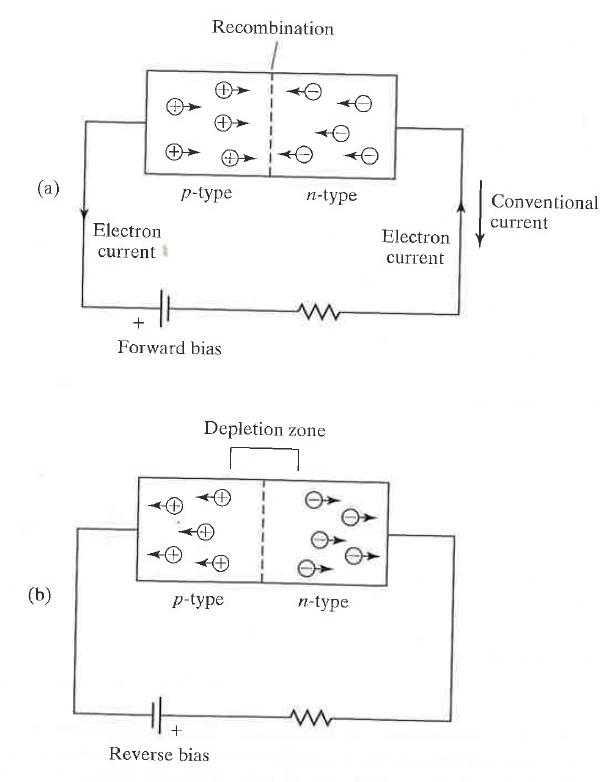
\includegraphics[scale=.7]{pnJunction.png}}
\caption{This is a diagram of a pn junction diode with current in different directions. In the clockwise current in a, the holes and electrons are constantly refreshed due to the applied potential, and the current can continuously flow. In the counterclockwise current, b, the applied potential increases the depeletion zone until the local electric field cancels out the applied potential and stops the flow of current.}
\label{pnJunction}
\end{figure}

The reason that current can only flow one direction can be seen in Figure \ref{pnJunction}. When there is a clockwise current as in Figure \ref{pnJunction}a, some holes from the p type and electrons from the n type combine at the interface and and produce heat.  So the diode loses electrons and holes at the interface, however the current pulls electrons from the p type resupplying the p type with holes. The converse happens in the n type so a current can flow indefinitely. This is known as forward bias. When the current flows counter-clockwise as in Figure \ref{pnJunction}b, the holes in the p type and the electrons in the n type flow away from the interface. This continues until the electric field due to the fixed impurity charges left behind is strong enough to balance the external field, causing the current to stop; this is known as reverse bias. 




\subsection{Transistors}
So now that we know what p type and n type doped semiconductors and pn junction diodes are, we can now talk about transistors. While there are many different types of semi conductors, the one that flash memory uses is the metal oxide semiconductor field effect transistor (MOSFET). A MOSFET, as seen in Figure \ref{mosfet}a consists of a p type silicon with two n type regions on each side, source and drain, and a metal gate separated from the semiconductor by an insulating oxide layer (typically SiO$_2$) in the middle. When no voltage is applied to the gate as seen in a, the MOSFET acts as two pn diodes, and so any voltage difference between the source and drain will reverse bias one of the two pn diodes so no current will flow. However, if a positive voltage is applied to the gate, the positive charge attracts electrons and repels holes as in Figure \ref{mosfet}b. If the voltage applied to the gate is above a certain threshold of around 1V, a thin layer of electrons will be formed under the oxide. Also known as the inversion layer, this creates a conducting channel between the source and drain, and the p type silicon acts as an n type allowing current to flow. This change created by the field from the gate is why it is called a field effect transistor. One advantage MOSFETS have over other transistors such as the Bipolar Junction Disorder is that the MOSFET requires nearly no current, so the input power is much less and there will be less issues with self-heating \cite{modernPhysics}.


\begin{figure}[H]
\centerline{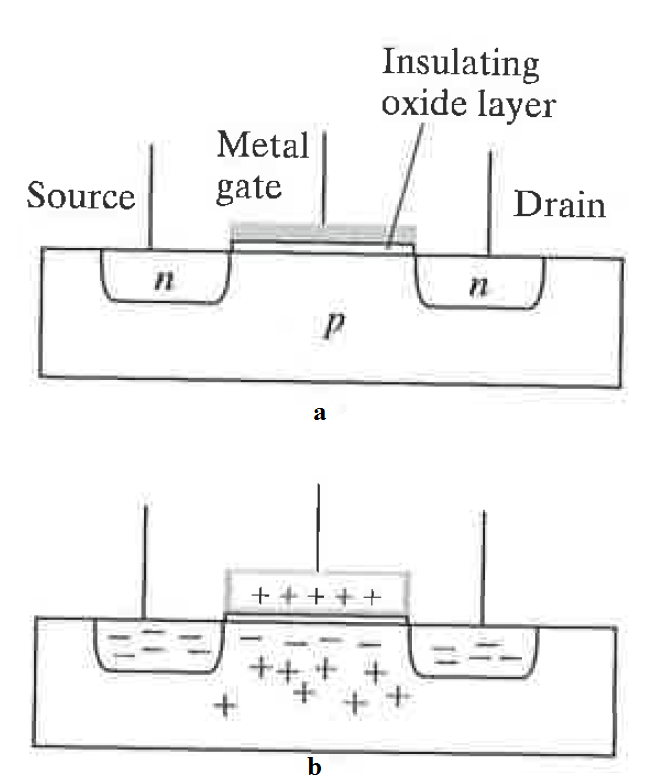
\includegraphics[scale=.45]{mosfet.png}}
\caption{Figure a is a normal MOSFET without any applied charge and thus acts an npn semiconductor and doesn't let current flow. In b, the positive charge on the metal gate cause electrons to build up along the oxide layer/semiconductor interface between the two n drops. This causes the semiconductor to turn into a n type semiconductor which allows current to flow.}
\label{mosfet}
\end{figure}

What is actually used to store bits is called the floating gate transistor. It is the same as the MOSFET except instead of only having one gate above the insulating oxide, you have another layer of insulating oxide on the other side of the gate followed by another gate called the control gate. So now the middle gate, also known as the floating gate, is electrically isolated due to the oxide layer on each side. Because of this, the only have to add and remove charge is through Fowler-Nordheim tunneling.  This means that when positive charge is stored on this gate, current will pass through and send a 1 and a 0 otherwise. Since the charges on the floating gate can not leave it without tunneling, that means that even when the transistor isn't powered, it will still store its memory. One peculiarity about flash memory is that it is structured in m blocks, typically powers of 2 and the number of blocks depend on the memory capacity. Also, each block is divided into k pages which is composed of bits created using floating gate transistors. The page is minimum programmable dimension, and the whole block is the minimum erasable area. One method used to increase storage density is to change from using single level cells (SLC) to multi level cells (MLC) and three level cells (TCL). SLC is the standard floating gate where it either outputs a 1 or 0 by dividing the gate into two possible states, current or no current.. However, the MLC stores 2 bits instead of one by dividing the gate into 4 possible states. While this has the benefit of doubling the storage density, it allows more room for error since the states are smaller and more difficult to distinguish. The oxide layer that was being used previously degraded after certain number of uses, and this degradation would become more visible on MLC drives first because they have to be able to disntinguish states more than SLC. However, advancements in both the oxide layer and also dynamic mapping of memory such that no one gate is used more than the other means that this have become more of a non issue.

By connecting the floating gate transistors in a way that resemebles a NAND gate such that bit line in Figure \ref{NAND} is only low if all the word lines are high. With this NAND flash, we can create all sorts of secondary storage: solid state drives, usb drives, and memory cards.

\begin{figure}[H]
\centerline{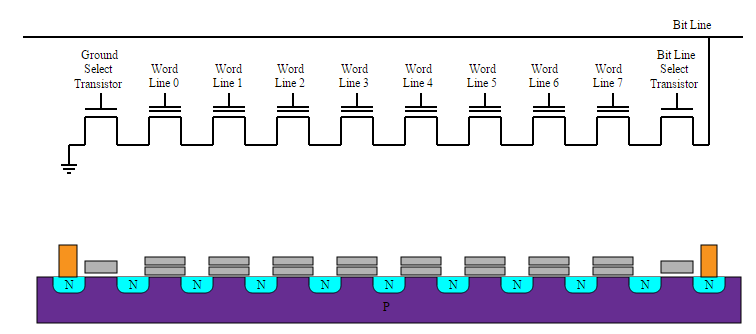
\includegraphics[scale=.45]{NAND.png}}
\caption{An example of how floating gate transistors are implemented in NAND flash. The name refers to the similarity with a NAND gate.}
\label{NAND}
\end{figure}

\section{Probe Based Storage}

While still very much in development, probe based storage could also offer an alternative to the more common storage systems such has hard drives and flash memory and compete with holographic storage. Based on the success of the scanning tunneling microscope (STM) and the atomic force microscope (AFM), there was much hope in using these new technologies to store massive amounts of data in much tinier scales than their traditional counterparts. While there is research being done on quite a few different approaches for probe based storage, such as magnetic storage medium, phase change medium, and ferroelectric approach, I will talk briefly about thermomechanical method of storing and retrieving data in nanometer-scale indentations in thin polymer films \cite{probe}.  While the write and read speed of a single probe is relatively slow, it can be greatly improved by instead using a large array of probes in parallel that all can read, write, and erase its spot. Instead of traditional rotating disks in hard drives, the storage medium is positioned by microelectromechanical system (MEMS) based x and y actuators, which typically have actuation distances of around 100 $\mu$m. In thermomechanical probe-based storage, 1s and 0s correspond to indentations or lack of indentations respectively. Also, these indentations are created by softening up the medium through local heating by the tip. As for the arrays themselves, a large array consisting of up to 4096 (64x64) cantilevers with tips and sensor has been successfully created using silicon micromachining techniques \cite{probe}.  However, having this many tips brings up other issues such as physically controlling that many tips accurately and also the large power consumption needed for that many tips. Nevertheless, probe based storage, with its ability to achieve ultrahigh densities of over 1 Tb/in$^2$, has potential to become the next popular storage method.


\section{Conclusion}
Digital data storage allows us to store our digital information. We're already able to store data at incredible densities or speeds, but as more and more information is being saved digitally we will need more and more dense and efficient ways to store our data. Since only two states are needed to store memory, it is very easy to find techniques to store memory like punch cards. However, it is quite difficult to find technique that are dense and efficient. As we've seen, there is continued improvements being made to current data storage techniques such as Blu-Ray discs and the change to perpendicular recording in hard drives. However, these are only short term solutions to our storage needs. Both holographic storage and probe storage are new techniques that each have the potential to store over 1 Tb/in$^2$, but they each have their own issues that currently keep them in the development stage. As our data needs keep growing, the technology needed to support that will continue to evolve as well.



\bibliographystyle{aip}
\bibliography{compsRef}



\end{document}
